\documentclass[12pt]{article}
\usepackage[breaklinks=true]{hyperref}
\usepackage[margin=1in]{geometry}
 
\usepackage{graphicx} %package to manage images
%\graphicspath{ {./images/} }

\usepackage{color}

\definecolor{pblue}{rgb}{0.13,0.13,1}
\definecolor{pgreen}{rgb}{0,0.5,0}
\definecolor{pred}{rgb}{0.9,0,0}
\definecolor{pgrey}{rgb}{0.46,0.45,0.48}

\usepackage{listings}
\lstset{language=Java,
  showspaces=false,
  showtabs=false,
  tabsize=2,
  breaklines=true,
  showstringspaces=false,
  breakatwhitespace=true,
  commentstyle=\color{pgreen},
  keywordstyle=\color{pblue},
  stringstyle=\color{pred},
  basicstyle=\ttfamily\small,
  frame=single,
  moredelim=[il][\textcolor{pgrey}]{$$},
  moredelim=[is][\textcolor{pgrey}]{\%\%}{\%\%}
}

\usepackage{setspace} % for \onehalfspacing and \singlespacing macros
\onehalfspacing 

\usepackage{etoolbox}
\AtBeginEnvironment{quote}{\singlespacing\small}

\title{\textbf{Exam Prep 2:} Another Deep Look at Our PPM Code}
\author{
	Melvyn Ian Drag
}
\date{\today}


\begin{document}
\maketitle

\begin{abstract}
In this class we'll discuss Pass-by-value vs. Pass-by-reference as well as take another look at how to set and unset individual bits in an \textit{int}. We will do these things as we look at our PPM manipulator code again.
\end{abstract}

\section{Garbage Collection, Primitives and References}
\subsection{Primitives}
Draw a picture showing how these are real ones and zeros in memory. When you pass a primitive to a function, the ones and zeros are copied to a new location. So, whatever you do to those ones and zeros only affects the copy. \textit{Draw a picture illustrating this and have the students draw it too.}

\subsection{Objects + References}
Whenever you do something like

\begin{lstlisting}
MyClass mc = new MyClass();
\end{lstlisting}

Java stores some 1s and zeros in memory to fit all the data needed by the my class object. It does one more thing - Java creates a reference. It stores an additional 4 bytes in memory that contain the location of that object in memory. The way those 4 bytes work is outside of the scope of this class - you need to understand pointers. Then, when you pass your object to a function, Java makes a copy of the thing being passed to the function...

But the thing that is copied is not the memory that corresponds to the MyClass object - the thing that is copied is the \textit{reference} to that thing. So, it you make a modification to the reference, you are actually modifying the object globally. \textit{Draw a picture and allow for a brief discussion}.

\subsection{Garbage Collection}
A major feature of Java comes from the fact that Java manages object references - you get \textbf{Garbage Collection}! \textit{Draw a picture of the RAM filling with stuff as more and more objects are ``newed up". why doesn't the computer crash? It doesn't crash because Java deletes the objects after using them so they don't fill your RAM. You may have sene your computer get really slow if you have too many browser tabs open - that's because there's no RAM left over and the computer gets `jammed up'.} This is one of the main features of the Java language - other languages  may not clean up the old 1s and 0s for you. Of course, the people who write languages without Garbage collection call the Java programmers babies who can't keep track of the memory usage of their programs. The Java programmers might fire back that the only reason that garbage collection was created is because the people who wrote programs with out GC wrote such sloppy code that Garbage collection became very imporant.
No matter your opinion, Garbage collection is one of the defining features of Java that is made possible by the fact that Java manages object references and not raw memory ( except with primitives ).

The fact that Java manages references to objects and not raw objects leads us to another defining feature of Java:

\section{Pass By Value}
From the \textit{javaworld.com} reference below:

\begin{quote}
Java does manipulate objects by reference, and all object variables are references. However, Java doesn't pass method arguments by reference; it passes them by value.
\end{quote}

What does that mean?!?

\begin{center}
\textbf{When you pass a parameter to a function in Java, the JVM copies the parameter into the function - it does not pass the actual object in.}
\end{center}

The learner is encouraged to study Java for another 6 months, then go learn about pointers in C++ and C to fully appreciate the difference between pass by value and pass by reference.

It is difficult to see that Java is pass by value, because all Java objects are references. The concept is simple, but difficult to explain without the learner understanding the way a few other programming languages work. Instead of explaining, I'll ask you to do the following assignment and see what strange things happen.

\subsection{How this relates to the PPM manipulating code from last week}
Look back at the function from the Week8 Code:

\begin{lstlisting}
	public static void ChangeWhiteToRed(int[][] inputArray){
		// ...
		// Note the void return type. 
		// Yet the inputArray[][] is still modified after this function
		// has been called. That may surprise you - you might have expected
		// that the inputArray would not be modified, and that you would
		// have to return an int[][] from the function. 
		// ...
	}
\end{lstlisting}

I want you to think more about this strange function. And so you can complete the following extra credit assignment.

\subsection{Extra Credit \#3}
Create a Java program with four functions:

\begin{enumerate}
\item \textit{public static void f1(float f)}
\item \textit{public static void f2(float[] fArr)}
\item \textit{public static void f3(CustomClass c)}
\item \textit{public static void f4(CustomClass2 c )}
\end{enumerate}

And write two classes

\begin{lstlisting}
public class CustomClass{
	public int x;
	CustomClass(int x){
		this.x = x;
	}	
}
\end{lstlisting}

and

\begin{lstlisting}
public class CustomClass2{
	public CustomClass cc;

	CustomClass2(CustomClass cc){
		this.cc = cc;
	}
}
\end{lstlisting}


The functions \textit{f1} - \textit{f4} should change the paramters passed to them. More specifically,

\begin{enumerate}
\item\textit{f1} should change the value of \textit{f}.
\item\textit{f2} should change the values in \textit{fArr}.
\item \textit{f3} should change the value of \textit{c.x}.
\item \textit{f4} should change the value of \textit{c.cc.x}.
\end{enumerate}


Check the parameter values before and after the function values ask Ask yourself:

\begin{center}
{\Large Which values were changed in the functions? Which ones did not change?}
\end{center}

You should see that the only value that is not changed in the function is the float f.

\subsection{Reference}
See this reference for more information: 
\url{https://www.javaworld.com/article/2077424/learn-java-does-java-pass-by-reference-or-pass-by-value.html}

\section{Setting Bits In an Int}
The essence of the midterm exam is to set a single bit in every int in an \textit{int[][]}. As we mentioned, in our steganography project we need to set the last bit in every int. More generally, something you might want to do in your code is set a bit, any one of the 32 bits in an int. How do you do that?

To set the last bit you do this:

\begin{lstlisting}
public int setLastBit(int i){
	return ( i | 0x00000001 );
}
\end{lstlisting}

to turn off the last bit in an int you would:

\begin{lstlisting}
public int zeroLastBit(int i){
	return ( i & 0xFFFFFFFE );
}
\end{lstlisting}

The above functions would be very useful to your midterm assignment\dots

\subsection{Extra Credit \#4a}
Write general implementations of the above. Implement the following function

\begin{lstlisting}
/**
 * Set a specified bit to either 1 or 0
 * 
 * @param originalValue - integer you want to modify
 * @param bitIndex - the bit ( 0 - 31 ) you want to change
 * @param value - New bit value. true for 1, false for 0. 
 */
public int setBit(int originalValue, int bitIndex, boolean value){
	// Implement me.
	// somehow create a newValue with the proper bit set to the proper val.
	return newValue;
}
\end{lstlisting}

The answer is here:
\url{https://stackoverflow.com/questions/4674006/set-specific-bit-in-byte}

\subsection{Extra Credit \#4b}
As the above is too simple - I've given a link with code you can copy and paste - you must do a little more work to earn these points. Copy the \textit{tricky} and \textit{main} functions from here: \url{https://www.javaworld.com/article/2077424/learn-java-does-java-pass-by-reference-or-pass-by-value.html}. Compile, run and explain the output to me.

\section{Also might be helpful for Midterm}

If, while doing the Midterm assignment, you need to extract the nth bit from a byte, you can do this:

\begin{lstlisting}
public static byte getBit(byte b, int index)
{
   return (byte)((b >> index) & 0x01);
}
\end{lstlisting}

You can verify that this works by checking the output for byte 0b01010101 = 0x55.

\lstinputlisting{BitExtractor.java}

Output:

\begin{figure}[h]
  \centering
    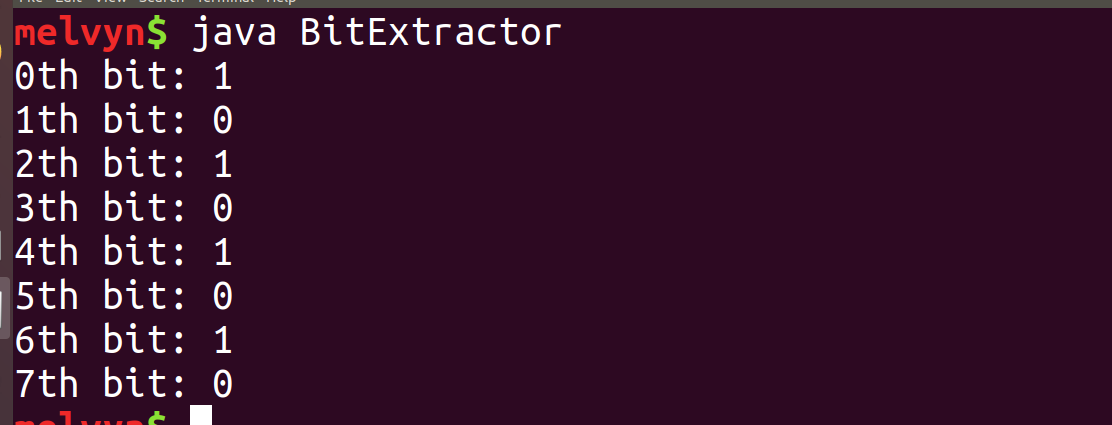
\includegraphics[width=0.5\textwidth]{bitExtractor.png}
  \caption{Showing the bits 0-7 being extracted from 0x55}
\end{figure}

\section{Midterm}

The midterm assignment is to:
\begin{enumerate}
\item Read an ASCII PPM image into an int[][]
\item Grab the bits one by one from an ASCII string
\item One by one, set the last bit in the (red?) channel of the PPM image using the bits from the step above.
\item Write the image out to a file.
\item Read the image back into memory.
\item Verify that the data was properly stored in the last bits of the red channel.
\end{enumerate}

Last week I gave a function that read a PPM into an int[][]. 

Last week we saw a function that writes the int[][] out to a PPM file.

Above you have functions for extracting bits and setting bits.

Good luck!

\section{Coming up next}
Over the next two weeks we'll look at some Java Collections.

\section{Final Exam Rough Draft}
Put on github. In the next few weeks we'll drill everything together to make sure you're ready.

\end{document}
